\documentclass{standalone}
\usepackage{tikz}
\usepackage{ctex,siunitx}
\setCJKmainfont{Noto Serif CJK SC}
\usepackage{tkz-euclide}
\usepackage{amsmath}
\usepackage{wasysym}
\usetikzlibrary{patterns, calc}
\usetikzlibrary {decorations.pathmorphing, decorations.pathreplacing, decorations.shapes,}
\begin{document}
\small
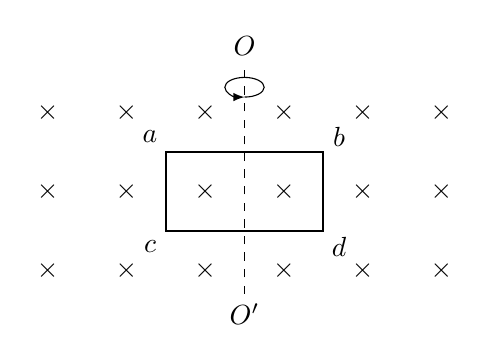
\begin{tikzpicture}[>=latex,scale=1]
	\foreach \x in{1,2,...,6}
		\foreach \y in {1,2,3}
		{
		   \node at (\x,\y) {$\times$};
		}
	\draw [thick](2.5,1.5) rectangle (4.5,2.5);
\draw [dashed](3.5,0.7)node[below] {$O'$}--(3.5,3.6)node[above] {$O$};
	\node at (2.3, 2.7) {$a$};	\node at (2.3, 1.3) {$c$};
	\node at (4.7, 2.7) {$b$};	\node at (4.7, 1.3) {$d$};
\draw[->] (3.5, 3.2) arc [start angle=-90, end angle=270, x radius=.25,y radius=.125];
\end{tikzpicture}
\end{document}